\documentclass[titlepage]{article}
\usepackage{listings}
\usepackage{graphicx}
\usepackage{color}
\usepackage{indentfirst}
\title{Criterion C | Mock Computer Science IA}
\author{Rohin Arya}
\date{Nov 30, 2022}

\begin{document}

\maketitle
\tableofcontents
\pagebreak

\section{Algorithmic Thinking: Managing a 2D Array}

In order to manage and display a map to the user, I used a 2D array. 2D Arrays are simple arrays that are comprised of other arrays such that targeting ARR[x][y] will return element y of array x. The following code shows the encapsulated instantiation of 2D Array \emph{map}:

\begin{lstlisting}[language=Java]
public class Map {
  private int[][] map;
  public Map(int x, int y) {
    map = new int[x][y];
  }
}
\end{lstlisting}

Further, traversing the array is done using nested for loops. The following code shows the \emph{generateMap()} method that generates a random map:

\begin{lstlisting}[language=Java]
public void generateMap() {
  for (int x = 0; x < map.length; x = x + 1) {
    for (int y = 0; y < map[x].length; y = y + 1) {
      int r = (int)(Math.random()*100);
      if (r < 50) {
        map[x][y] = 2;
      }
      else if (r < 75) {
        map[x][y] = 1;
      }
      else {
        map[x][y] = 0;
      }
    }
  }
}
\end{lstlisting}

Shown above, the \emph{generateMap()} method uses a nested for loop to traverse the 2D array. A random number between 0 and 100 is generated in order to randomly fill the 2D Array with tile IDs.

In order to print the map to the user, another set of nested loops are used to traverse the array. The following code shows part the overridden \emph{paintComponent()} method that helps print the map to the user:

\begin{lstlisting}[language=Java]
for (int y = 0; y < map.getY(); y = y + 1) {
  for (int x = 0; x < map.getX(); x = x + 1) {
    if (map.getValue(x, y) == 0) {
      g.setColor(Color.GREEN);
    }
    ...
    g.fillRect(x*10, y*10, x*10 + 10, y * 10 + 10);
  }
}
\end{lstlisting}

The 2D arrays are traversed row-majorly, meaning that the first for loop traverses the rows and the second for loop traverses the columns. \emph{y} is defined as the row and \emph{x} is defined as the column. The coordinate of the pixel is effectively \emph{(x, y)}. Thus, when filling in the area of the GUI with color, \emph(x) is passed as the x-coordinate and \emph(y) is passed as the y-coordinate. The width and height of the rectangle are set to 10 pixels, thus each value is multiplied by 10. The photo shows the map generated by the code above:

\vspace*{5mm}

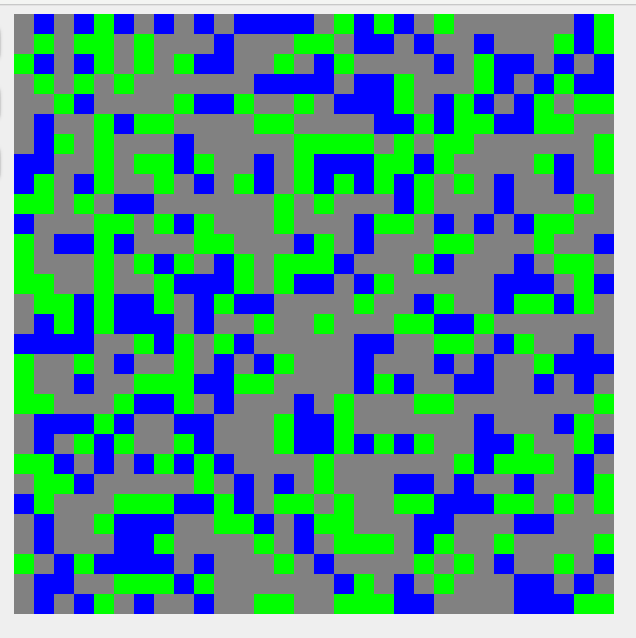
\includegraphics[width=\linewidth]{images/SCR-20221202-hfj.png}


\pagebreak
\section{Algorithmic Thinking: Something with Unlimited Map}
\pagebreak
\section{Technique: Class Structure}

Class structure is the organization of classes and methods in a program. In order to organize my code, I used the following class structure:

\emph{Map} - Used to generate and store the map. It contains the 2D array and methods to modify it.

\emph{Player} - Used to store the player's position and methods to modify it.

\emph{GameMain} - Entry point used to generate the GUI, handle user input, and update the display.

The purpose of this class structure is to separate the code into different classes that are responsible for different tasks. This allows for easier debugging and modification of the code. The entry point of the program is in \emph{GameMain.java}:

\begin{lstlisting}[language=Java]
public static void main(String[] args) {
  GameMain gm = new GameMain();
}
\end{lstlisting}

Here, a new instance of GameMain is created and the constructor is called. The constructor then starts creating the GUI:

\begin{lstlisting}[language=Java]
public GameMain() {
  map = new Map(30,30); // Make map
  frame = new JFrame(); // Construct graphic elements
  panel = new JPanel();
  ...
\end{lstlisting}

The benefit of creating a dedicated class for the game is that multiple instances of the game can be created and managed. This includes potential future functionality of comparing games states, and saving and loading games.

\vspace*{5mm}
(UML DIAGRAM HERE ON CODE COMPLETION)
\vspace*{5mm}

Another important aspect of class structure is the use of access modifiers. Access modifiers are used to restrict access to certain methods and variables. For example, the \emph{map} variable in the \emph{GameMain} class is private. This is an example of encapsulation, meaning that it can only be accessed by methods in the same class.

\pagebreak
\section{Technique: Writing and Reading Data}

In order to save and load the game, I used the \emph{File} class. The following code shows the \emph{saveGame()} method that saves the game to a file:

\pagebreak
\section{Technique: Interfaces}

Interfaces in Java are used to define a set of methods that a class must implement. For example, the \emph{ActionListener} interface is used to define the methods that a class must implement in order to handle key events. The following code shows the \emph{GameMain} class implementing the \emph{ActionListener} interface:

\begin{lstlisting}[language=Java]
private ActionListener action = new ActionListener() {
  @Override public void actionPerformed(ActionEvent e) {
    if (e.getSource() == attackBTN) {
      ...
    }
    else {
      ...
    }
  }
}
\end{lstlisting}

A similar interface process is used in the \emph{KeyListener} and \emph{JPanel} instances. Interfaces are useful for defining contracts or standards within the code, ensuring that interfaced classes contain certain methods. This allows for easier development and extensibility of the code.
The \emph{@Override} annotation is used in a Java to indicate that a method is intended to override a method with the same name and parameters in an interface. 

This annotation can help prevent errors by indicating to the compiler that the overridden method exists and has the correct signature. Method signature refers to the combination of name, type, and parameters of a method.
\begin{lstlisting}
private KeyListener kl = new KeyListener() {
  @Override public void keyTyped(KeyEvent e) {
    ...
  }
  ...
}
\end{lstlisting}

A similar process is used for the \emph{KeyListener} instance shown above, where the \emph{keyTyped()} method is overridden.





\pagebreak
\end{document}